%%%
%%% Document class and page properties
%%%

\documentclass{IIBproject}

% Set margin size
\usepackage[margin=2.5cm]{geometry}

% Set table of contents depth
\setcounter{tocdepth}{2}

%%%
%%% Standard packages in alphabetical order
%%%

% Use the AMS math package for special fonts such as mathbb (included in the amssymb package
% coming with ams math), inline text in equations, etc.
\usepackage{amsmath}
\usepackage{amssymb}

% Use the calc package for infix arithmetic
\usepackage{calc}

% Use BibTeX for bibliography management, use the hyperref package to include URLs in the entries
\usepackage{cite}
\usepackage{url}

% Color text
\usepackage{color}

% Sets 1.5 line spacing
\usepackage{setspace}
\onehalfspacing

% Provides formatting of numbers (here used for thousands' separators)
\usepackage{siunitx}

% Use the tikz package for drawing
\usepackage{tikz}

% Provides robust spaces after commands
\usepackage{xspace}

%%%
%%% Commands
%%%

% Define macros for correct spacing after abbreviations, source: http://tex.stackexchange.com/a/15017
\newcommand*{\ie}{i.e.\@\xspace}

% Abbreviations which can occur at the end of the sentence cannot duplicate the following dot
\makeatletter
\DeclareRobustCommand*{\AbbreviationWithDot}[1]{\@ifnextchar{.}{#1}{#1.\@\xspace}}
\DeclareRobustCommand*{\pmf}{\AbbreviationWithDot{p.m.f}}
\makeatother

% Placeholder for parts of the report to be finished later
\DeclareRobustCommand{\later}{\textcolor{red}{\textbf{(?)}}\@\xspace}

% Notes to be discussed with supervisor/thought about later
\DeclareRobustCommand{\noteSelf}[1]{\textcolor{red}{#1}}

%%%
%%% Drawing
%%%

% Define a new tikz style for drawings left-closed intervals: [i], notice that the heads are centred exactly on the start and end coordinates of the line
\usetikzlibrary{decorations.markings}
\tikzset{
    i/.style={
        shorten >=#1,
        decoration={
            markings,
            mark={ at position 0 with {\filldraw[solid] circle [radius=#1];} },
            mark={ at position 1 with {\draw[solid] circle [radius=#1];} }
        },
        postaction=decorate
    },
    i/.default=1.5pt
}

% Define macros for drawing a vertical interval, the arguments are always:
%	(#1,#2)	- start position
%	(0,#3)	- length vector
%	(#4,#5)	- beginning and end of the interval, normalised between 0 and 1
%	#6		- line style
%	#7		- position of the label ("left" or "right") if the interval is labelled
\newcommand{\interval}[6] {
	\draw[#6] [i] (#1,#2+#4*#3) -- (#1,#2+#5*#3);
}

\newcommand{\intervalTopLabel}[7] {
	\interval{#1}{#2}{#3}{#4}{#5}{#6}
	\node[#7] at (#1,#2+#5*#3) {\footnotesize #5};
}

\newcommand{\intervalBottomLabel}[7] {
	\interval{#1}{#2}{#3}{#4}{#5}{#6}
	\node[#7] at (#1,#2+#4*#3) {\footnotesize #4};
}

\newcommand{\intervalBothLabels}[7] {
	\intervalBottomLabel{#1}{#2}{#3}{#4}{#5}{#6}{#7}
	\node[#7] at (#1,#2+#5*#3) {\footnotesize #5};
}

%%%
%%% Document
%%%

\begin{document}

% Title page
\thispagestyle{empty}
\author{Konrad Komorowski (CHU)}
\title{Hiding Secrets in Plain Text}
\projectgroup{F}
\maketitle

% Summary and table of contents
\thispagestyle{empty}
\begin{abstract}
Lorem ipsum dolor sit amet, consectetur adipisicing elit, sed do eiusmod tempor incididunt ut labore et dolore magna aliqua. Ut enim ad minim veniam, quis nostrud exercitation ullamco laboris nisi ut aliquip ex ea commodo consequat. Duis aute irure dolor in reprehenderit in voluptate velit esse cillum dolore eu fugiat nulla pariatur. Excepteur sint occaecat cupidatat non proident, sunt in culpa qui officia deserunt mollit anim id est laborum.
\end{abstract}

\tableofcontents

% Contents
\pagestyle{plain}

\newpage
\section{Technical abstract}

Lorem ipsum.

\newpage
\section{Introduction}

Lorem ipsum.

\subsection{Aim}

\subsection{Overview of steganography}

\subsection{High level description of the stegosystem}

\newpage
\section{The interval algorithm}

The interval algorithm \cite{hanhoshi1997} provides a means of sampling from an arbitrary stochastic process (target) given an input sequence from a different arbitrary stochastic process (source). The algorithm is very similar to arithmetic coding -- it also uses successive refinements of the $[0,1)$ interval to map sequences.

The sequence mapping algorithm starts by mapping the empty sequence $[~]$ to the interval $[0,1)$. For any sequence, its interval is partitioned into subintervals corresponding to the sequence extended by a single term. The size of each interval is chosen to be proportional to the probability of the last term occurring given the preceding sequence. The order of the subintervals does not matter, but needs to be consistent if reverse mapping from an interval to a sequence is to be performed. By the chain rule of probability, the size of the resulting interval is equal to the probability of observing its sequence. Consequently, only sequences of non-zero probability can be mapped. For a more detailed overview of arithmetic coding see \cite{coverthomas:sfecoding}.

The interval algorithm works by continuously mapping the observed input sequence to successive intervals defined by the stochastic model of the source. In parallel, the intervals are reverse mapped to an output sequence according to the stochastic model of the target. Terms of the output sequence can be generated as long as its interval is a superinterval of the input sequence interval. See Fig.~\ref{fig:interval_algorithm} for an example of the procedure.

\begin{figure}[h]
	\centering

	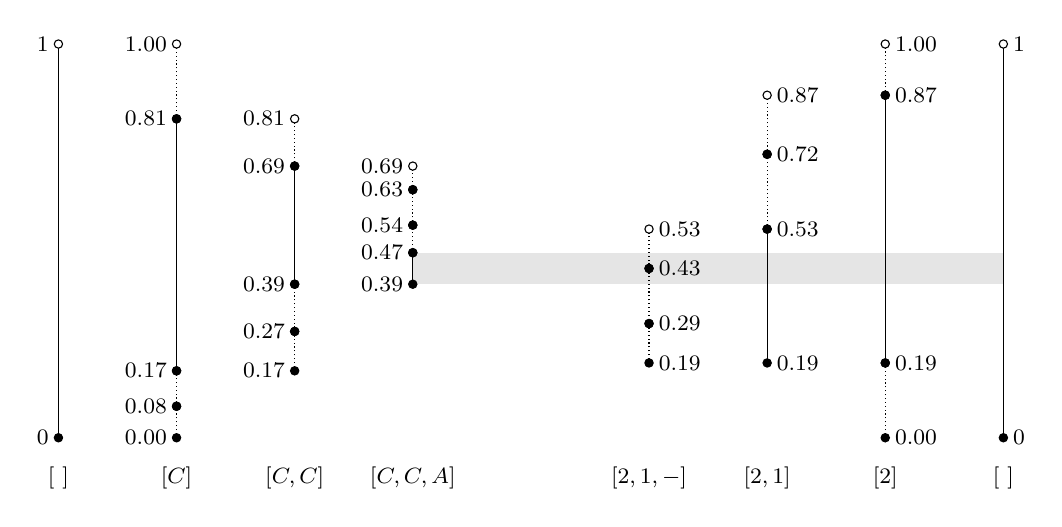
\begin{tikzpicture}[scale=0.05]
		% Final interval range
		\fill [opacity=0.1] (-30,0.39*100) rectangle (120,0.47*100);

		% Input side
		\intervalBothLabels{-120}{0}{100}{0}{1}{solid}{left}
		\node[below] at (-120,-5) {\footnotesize $[~]$};

		\intervalBothLabels{-90}{0}{100}{0.81}{1.00}{densely dotted}{left}
		\intervalBottomLabel{-90}{0}{100}{0.17}{0.81}{solid}{left}
		\intervalBottomLabel{-90}{0}{100}{0.08}{0.17}{densely dotted}{left}
		\intervalBottomLabel{-90}{0}{100}{0.00}{0.08}{densely dotted}{left}
		\node[below] at (-90,-5) {\footnotesize $[C]$};

		\intervalBothLabels{-60}{0}{100}{0.69}{0.81}{densely dotted}{left}
		\intervalBottomLabel{-60}{0}{100}{0.39}{0.69}{solid}{left}
		\intervalBottomLabel{-60}{0}{100}{0.27}{0.39}{densely dotted}{left}
		\intervalBottomLabel{-60}{0}{100}{0.17}{0.27}{densely dotted}{left}
		\node[below] at (-60,-5) {\footnotesize $[C,C]$};

		\intervalBottomLabel{-30}{0}{100}{0.39}{0.47}{solid}{left}
		\intervalBottomLabel{-30}{0}{100}{0.47}{0.54}{densely dotted}{left}
		\intervalBottomLabel{-30}{0}{100}{0.54}{0.63}{densely dotted}{left}
		\intervalBothLabels{-30}{0}{100}{0.63}{0.69}{densely dotted}{left}
		\node[below] at (-30,-5) {\footnotesize $[C,C,A]$};

		% Output side
		\intervalBothLabels{120}{0}{100}{0}{1}{solid}{right}
		\node[below] at (120,-5) {\footnotesize $[~]$};

		\intervalBothLabels{90}{0}{100}{0.87}{1.00}{densely dotted}{right}
		\intervalBottomLabel{90}{0}{100}{0.19}{0.87}{solid}{right}
		\intervalBottomLabel{90}{0}{100}{0.00}{0.19}{densely dotted}{right}
		\node[below] at (90,-5) {\footnotesize $[2]$};

		\intervalBothLabels{60}{0}{100}{0.72}{0.87}{densely dotted}{right}
		\intervalBottomLabel{60}{0}{100}{0.53}{0.72}{densely dotted}{right}
		\intervalBottomLabel{60}{0}{100}{0.19}{0.53}{solid}{right}
		\node[below] at (60,-5) {\footnotesize $[2,1]$};

		\intervalBothLabels{30}{0}{100}{0.43}{0.53}{densely dotted}{right}
		\intervalBottomLabel{30}{0}{100}{0.29}{0.43}{densely dotted}{right}
		\intervalBottomLabel{30}{0}{100}{0.19}{0.29}{densely dotted}{right}
		\node[below] at (30,-5) {\footnotesize $[2,1,-]$};

	\end{tikzpicture}

	\caption{\label{fig:interval_algorithm} Example run of the interval algorithm. On the left, an input sequence $[C,C,A]$ from the source process gets mapped to $[0.39,0.47)$. On the right, this interval allows to generate up to 2 terms of an output sequence from the target process, \ie $[2,1]$, which correspond to $[0.19,0.53)$. Note that it is not possible to generate more terms of the output sequence, as neither $[0.19,0.29)$ nor $[0.29,0.43)$ nor $[0.43,0.53)$ is a superinterval of $[0.39,0.47)$.}

\end{figure}

\newpage
\section{Statistical language models}

\subsection{Standard theory and notation}

The notation and theory in this section is mostly based on \cite{4f11:statistical_language_models, 4f11:smt_systems, coursera:nlp}.

\subsubsection{Text as the output of a stochastic process}

A string $\mathbf w$ of length $L$ can be regarded as a sequence of \emph{tokens} $w_l$. Tokens are atomic elements of text such as words or punctuation marks.

\begin{equation}
\mathbf w = [ w_1, \dots, w_L ] \equiv w_1^L
\end{equation}

$\mathbf w$ can be regarded as an $L$-dimensional vector of jointly distributed random variables $w_l \in \{1, \dots, M\}$, where $M$ is the number of distinct tokens. According to the chain rule of probability, we can factorise $P(\mathbf w)$ in the following way:

\begin{equation}
\label{eq:exact_string_probability}
P(\mathbf w) = \prod_{l=1}^{L} P( w_l | w_1^{l-1} )
\end{equation}

Even though Eq.~\ref{eq:exact_string_probability} gives a convenient formulation of language as a stochastic process, it is computationally intractable. The conditional probabilities need to be stored in tables. Conditional probability table of just the last token would have $M^L$ entries. With $M \approx 10^6$ and $L \approx 10$, this number very quickly becomes prohibitively large.

\subsubsection{$N$-gram language models}

The usual solution is to restrict the size of the context to $N-1$ previous tokens, resulting in an approximate $N$-gram language model:

\begin{equation}
\label{eq:ngram_string_probability}
P(\mathbf w) \approx P_{\text{$N$-gram}}(\mathbf w) \equiv \prod_{l=1}^{L} P( w_l | w_{l-N+1}^{l-1} )
\end{equation}

\subsubsection{Estimating parameters}

Eq.~\ref{eq:ml_conditional_token_probability} is the ML (maximum likelihood) estimate of conditional probability of $w_l$ in an $N$-gram model. $f(\cdot)$ is the number of occurrences of a particular sequence of tokens in the training dataset.

\begin{equation}
\label{eq:ml_conditional_token_probability}
\hat P( w_l | w_{l-N+1}^{l-1} ) = \frac {f(w_{l-N+1}^l)} {f(w_{l-N+1}^{l-1})}
\end{equation}

A problem with Eq.~\ref{eq:ml_conditional_token_probability} is that most $N$-gram counts will be zero. For example, a $5$-gram model with $M \approx 10^6$ will have $M^L \approx \left( 10^6 \right)^5 = 10^{30}$ distinct $N$-grams. For every possible $5$-gram sequence to occur at least once, the training set would need to consist of $\ge 10^{30}$ tokens. Currently largest available dataset is based on $\approx 3.6 \times 10^{11}$ English words. \cite{googlengrams2011} As a result, a large number of grammatically correct sentences would have 0 probability.

\subsubsection{Limiting database size, discounting and back-off}

A standard way of dealing with this problem is by introducing \emph{discounting} and \emph{backing-off} the model. In addition, $N$-grams with counts below a threshold $C$ are sometimes discarded from the database to conserve storage space. Conditional distribution of the $l$th token becomes:

\begin{equation}
	\label{eq:conditional_token_probability_with_backoff}
	P( w_l | w_{l-N+1}^{l-1} ) =
	\begin{cases}
		d (w_{l-N+1}^l) ~ \frac {f\left(w_{l-N+1}^l \right)} {f\left(w_{l-N+1}^{l-1} \right)} & \text{if $f(w_{l-N+1}^l) \ge C$},\\
		\alpha (w_{l-N+1}^{l-1}) ~ P( w_l | w_{l-N+2}^{l-1} ) & \text{otherwise}.
	\end{cases}
\end{equation}

$d(\cdot)$ and $\alpha(\cdot)$ return the discount and back-off weights -- scaling factors used to ensure that Eq.~\ref{eq:conditional_token_probability_with_backoff} is a valid \pmf. Intuitively, they reduce the mass assigned to observed $N$-grams to accommodate for estimates of order $N-1$ and lower. $d(\cdot)$ and $\alpha(\cdot)$ are hard to choose or compute -- there exist many different schemes motivated by linguistics and statistics. Examples include Good-Turing smoothing,\cite{good1953} Kneser-Ney smoothing,\cite{kneserney1995} or stupid back-off.\cite{brants2007} All exhibit various levels of complexity and the latter does not even return a valid \pmf's.

\subsection{Sources of natural language statistical data}

\subsubsection{COCA}

\subsubsection{Google Books Ngrams}

\newpage
\section{Detailed description of the stegosystem}

Lorem ipsum.

\subsection{Source -- plaintext concatenated with randomness}

\subsection{Target -- English language model}

\subsection{Storing length of plaintext}

\subsubsection{Universal coding of plaintext length}

\subsubsection{EOF symbol}

\subsection{Sufficient length of the output interval}

\subsection{Secrecy}

\newpage
\section{Implementation}

Lorem ipsum.

\subsection{Language model}

\subsubsection{Mining the Google Books Ngrams Database}

\subsubsection{Efficient computation of conditional probabilities}

\subsection{Plaintext to stegotext translation using the interval algorithm}

\newpage
\section{Security vulnerabilities}

Lorem ipsum.

\subsection{Telling stegotext from covertext}

\subsubsection{Plaintext length declaration incompatible with interval size}

If the plaintext length declaration is longer than the maximum length of plaintext that can be recovered from the potential stegotext, we know the message was covertext.

Conversely -- how often does a compatible length declaration indicate stegotext? If almost always, then the system is flawed.

\newpage
\section{Theoretical considerations}

Lorem ipsum.

\subsection{Rate of the system}

\subsection{Entropy of the language model and its effect on stegotext length}

Use the bounds from Han \& Hoshi's paper.

\newpage
\section{Interesting questions}

Lorem ipsum.

\subsection{How many bits of information stored per word, sentence, tweet?}

\subsubsection{Dependence on the entropy of the language model}

\newpage
\footnotesize
\bibliographystyle{unsrt}
\bibliography{../bibliography}

\newpage
\appendix

\section{First appendix}

\end{document}